\documentclass[a4paper,12pt]{article}
\usepackage[margin=0.7in]{geometry}
\usepackage{algorithm}
\usepackage{algpseudocode}
\usepackage{tikz}
\usepackage[cm-default]{fontspec}
\usepackage[hidelinks]{hyperref}
\usepackage{xunicode}
\usepackage{xltxtra}
\usepackage{amsfonts, amsmath}
\setlength{\tabcolsep}{0.6em} % for the horizontal padding
{\renewcommand{\arraystretch}{1.5}% for the vertical padding
\algnewcommand{\LineComment}[1]{\State \(\triangleright\) #1}
\usepackage{amsthm}

\usepackage[utf8]{inputenc}
\newtheorem*{theorem}{Θεώρημα}
\newtheorem*{lemma}{Λήμμα}

\usepackage[greek]{babel}
\usepackage{xgreek}
\usepackage{algpseudocode, listings}
\setmainfont{Times New Roman}
\usepackage{titling}
\newcommand{\N}{\ensuremath{\mathbb N} }
\newcommand{\A}{\ensuremath{\mathcal A} }
\newcommand{\pset}[1]{\ensuremath{\mathcal P( #1 )}}
\newcommand{\pr}[1]{\ensuremath{\mathbb P [ #1 ]}}
\newcommand{\ev}[1]{\ensuremath{\mathbb E [ #1 ]}}
\newcommand{\R}{\ensuremath{\mathbb R}}
\newcommand{\opt}{\textsc {Opt}}

\lstset{basicstyle=\footnotesize\ttfamily,breaklines=true}

\usepackage{graphicx}


\title{ \textbf{Τεχνητή Νοημοσύνη}  \\ 2o Προγραμματιστικό Θέμα \\ Αναφορά Εργασίας \\ \small{Ακ. Έτος 2018-2019}}
\author{\textbf{Μέλη ομάδας (αλφαβητικά)} \\ Εμμανουήλ Παναγιώτου (03115079) -- \texttt{el15079@mail.ntua.gr} \\  Μάριος Παπαχρήστου (03115101) -- \texttt{papachristoumarios@gmail.com} \\ \noindent\rule{0.9\textwidth}{1pt}}
\date{\emph{"It's going to be interesting to see how society deals with artificial intelligence, but it will definitely be cool". --Colin Angle}} 


\begin{document}

\maketitle

\section{Σκοπός Εργασίας} 

Σε αυτή την εργασία υλοποιούμε το βασικό κορμό μιας ευφυούς υπηρεσίας εξυπηρέτησης πελατών ταξί. Συγκεκριμένα,θεωρούμε ότι υπάρχει ένας πελάτης που βρίσκεται σε μια ορισμένη τοποθεσία, ο οποίος διαθέτει κινητό τηλέφωνο με GPS και επιθυμεί να καλέσει ένα ταξί. Η υπηρεσία διαθέτει μια βάση δεδομένων με όλα τα διαθέσιμα ταξί και τη γεωγραφική θέση στην
οποία βρίσκονται κάθε χρονική στιγμή, η οποία θεωρητικά θα πρέπει να ανανεώνεται συνεχώς. Η υπηρεσία θα πρέπει να εντοπίζει και να ειδοποιεί το ταξί που μπορεί να μεταβεί πιο γρήγορα στη θέση του πελάτη ώστε να τον εξυπηρετήσει. Ο χάρτης δίνεται απο δειγματοληπτημένα σημεία οδών από την πόλη της Αθήνας και ο τρόπος εύρεσης της βέλτιστης επιλογής γίνεται με τη χρήση του αλγορίθμου Α* με τη δυνατότητα επιλογής πολλών εναλλακτικών διαδρομών (similar ETA).  Στη συνέχεια ο πελάτης πρέπει να μετακινηθεί βέλτιστα στον προορισμό του.

Στη συγκεκριμένη περίπτωση θα παρέχεται ένας πυρήνας σε Java με τις κύριες λειτουργίες του αλγορίθμου, ενώ όλη η γνώση των πρακτόρων προέρχεται από κατηγορήματα σε γλώσα Prolog. Για την διασύνδεση Java και Prolog έχει χρησιμοποιηθεί η βιβλιοθήκη JIProlog. 

\section{Εκτέλεση εργασίας}

Στην εργασία παρέχεται ένα Makefile για την εκτέλεση των σεναρίων. Για να εκτελέσουμε όλη την εργασία χρησιμοποιούμε την \texttt{make all}. Η κύρια κλάση βρίσκεται στο \texttt{Graph.java}. 

\section{Οργάνωση και Διάρθρωση Γνώσης για τον Κόσμο} 

Θεωρώντας ότι τα ταξί και οι πελάτες ζουν σε ένα κόσμο με κάποιες ιδιότητες, μπορούμε να ορίσουμε μια σειρά από κατηγορήματα σε Prolog που αναπαριστούν όλα αυτά τα σενάρια. Συγκεκριμένα, θεωρούμε ότι ο χάρτης αναπαρήσταται από ένα κατευθυνόμενο γράφημα $G(V, E)$ όπου το κατηγόρημα \texttt{next/4} αναφέρεται σε ακμή του γραφήματος, το κατηγόρημα \texttt{lines/20} σε οδούς στο δρόμο, το κατηγόρημα \texttt{taxis/10} στα ταξί, το κατηγόρημα \texttt{client/9} στους πελάτες και το κατηγόρημα \texttt{traffic/5} στην κίνηση της εκάστοτε οδού. Τα κατηγορήματα αυτά κατασκευάζονται από τα αρχεία CSV που μας παρέχονται και την κλάση \texttt{FactGenerator}. Παραθέτουμε μερικά παραδείγματα

\begin{lstlisting}[language=prolog]
traffic(5203817,mask,[09:00-11:00=high,13:00-15:00=medium,17:00-19:00=high], mask,mask).
client(0,23.733912,37.975687,23.772518,38.012301,20:00,3,greek,1).
taxis(23.789114,38.032908,130,no,1-4,[greek,english],8.3,yes,subcompact,mask).
\end{lstlisting}  

όπου έχουμε χρησιμοποιήσει το άτομο \texttt{mask} για τους χαρακτήρες που δεν είναι ASCII ή δεν υπάρχει πληροφορία. 

Στη συνέχεια ορίζουμε κατηγορήματα που αφορούν μεταβάσεις και λοιπές πληροφορίες για τον κόσμο στο αρχείο \texttt{world.pl} όπως φαίνεται παρακάτω και στο οποίο κάνουμε consult όλη τη βάση γνώσης. 

\lstinputlisting[language=Prolog]{../../src/world.pl}

Εδώ παρατηρούμε ότι μπορούμε να επιτελέσουμε διάφορες λειτουργίες, όπως να βρούμε τα υποψήφια ταξί στόχους, να βρούμε γείτονες κόμβους που η μετάβαση δεν έχει συνωστισμό μια συγκεκριμένη ώρα κτλ. Στη συνέχεια, δημιουργούμε έναν wrapper μεταξύ του \texttt{world.pl} και της Java λειτουργικότητας μέσω της βιβλιοθήκης JIProlog στην κλάση \texttt{Prolog.java}. 

\section{Αντικειμενοστραφής Σχεδιασμός} 

Η παρούσα εργασία αναπτύχθηκε σε γλώσα Java, με γνώμονα τον αντικειμενοστραφή σχεδιασμό. Χρησιμοποιήθηκαν κλάσεις για τα Ταξί (Taxi), τους Πελάτες (Client), τις Κορυφές (Node), τις ακμές (Edge), τους εκτιμητές για τον Α* (Estimator) και τον συνολικό γράφο (Graph). Τo parsing των κορυφών γίνεται μέσω της κλήσης των κατάλληλων μεθόδων του wrapper. Τέλος χρησιμοποιήθηκε μια κλάση (Visual) για την παραγωγή των αρχείων KML ώστε να γίνεται η απεικόνιση των αποτελεσμάτων στον χάρτη. Για τις δομές δεδομένων χρησιμοποιήθηκαν επίσης κλάσεις των standard βιβλιοθηκών της Java. 

\section{Δημιουργία Γραφήματος}

Ο γράφος χτίζεται on-line με τη χρήση των κατάλληλων κατηγορημάτων που υπάρχουν στο \texttt{world.pl} για την λήψη των adjacent κόμβων ενός κόμβου $u$ μέσω της κλήσης της μεθόδου \texttt{next}. Το μήκος κάθε ακμής $\{u, v\} \in E$ τίθεται ίσο με την γεωγραφική απόσταση σε km δηλαδή 

$$w(u, v) = \mathrm{geo}(u, v) = 111.18957696 \times \arccos \left [ \sin \phi_u \sin \phi_v + \cos \phi_u \cos \phi_v \cos (\theta_u - \theta_v) \right ]$$





\section{Αλγόριθμος Α*}

\subsection{Περιγραφή Αλγορίθμου}
Για την υλοποίηση του Α* χρησιμοποιήθηκαν δύο hashtables για να κρατήσουμε τις $f(v)$ και $g(v)$. Επίσης χρησιμοποιήθηκε ένα HashSet για τη διατήρηση του κλειστού συνόλου και μια ουρά προτεραιότητας \texttt{PriorityQueue<Estimator>} στην οποία τηρούταν το μέτωπο αναζήτησης (ανοικτό σύνολο). Κάθε φορά, από το μέτωπο αναζήτησης αφαιρούνταν ο κόμβος με την ελάχιστη τιμή $$f(v) = g(v) + h(v)$$ όπου $h(v)$ η ευριστική συνάρτηση. Αν ο $v$ ήταν στόχος τότε η αναζήτηση τερμάτιζε. Σε κάθε άλλη περίπτωση ο αλγόριθμος έκανε relax στις κορυφές στις οποίες βελτιώνονταν το $g(v)$. 

\subsection{Ευριστική Συνάρτηση}

Δεδομένης της γεωμετρίας της πόλης, η ευριστική συνάρτηση που διαλέξαμε είναι η Νόρμα Ταξί $L_1$ από τον κοντινότερο στόχο με τύπο 

$$h(v) = \min_{g \in G} h_g(v)$$

όπου $G = \{ g \in V \mid g \text{ στόχος} \}$ με $$h_g(v) = \lambda \mathrm{geo}(v, g) \qquad \lambda \le 1$$
 
Στη δική μας υλοποίηση θέσαμε $\lambda=0.9$. Για να επιστρέψει σωστά αποτελέσματα ο Α* θα πρέπει η ευριστική συνάρτηση να υποεκτιμά το πραγματικό κόστος προς το στόχο.
\subsection{Αποθήκευση Διαδρομών} 

Για να τηρήσουμε τις διαδρομές χρησιμοποιούμε ένα \texttt{Hashtable<Node, ArrayList<Pair>>} και σε κάθε relaxation προσθέτουμε στη λίστα την τιμή που βρίσκουμε (η οποία μικραίνει συνεχώς). Ο πίνακας κατακερματισμού θα χρησιμεύσει στην εκτύπωση των συντομότερων διαδρομών. Ο κατευθυνόμενος υπολειμματικός γράφος $H$ είναι DAG. Κάνοντας μια αναζήτηση από την κορυφή--στόχο στην αρχή μπορούμε να φτιάξουμε το γράφημα των ισοδύναμων βέλτιστων διαδρομών για τις τιμές των εκτιμήσεων της πραγματικής απόστασης του κάθε κόμβου σε κάθε χρονική στιγμή με τη βέλτιστη (συγκλίνουσα) εκτίμηση. Για τις ισοδύναμες διαδρομές έχουμε επιτρέψει κάποιο tolerance $\epsilon$ (της τάξης των 0.001km).  

\subsection{Αξιολόγηση Αλγορίθμου} 

Ο αλγόριθμος Α* βρίσκει τη βέλτιστη λύση αν η ευριστική συνάρτηση $h(v)$ \textbf{υποεκτιμά το πραγματικό κόστος προς τον κοντινότερο στόχο}. Ο πίνακας κατακερματισμού για τους γονείς (parent) επιτρέπει σε κάθε έναν κόμβο να έχει γονείς εντός μιας ακρίβειας $\epsilon$ από τη βέλτιστη τιμή $g(v)$. Το συγκεκριμένο πρόβλημα πληροί τις προϋποθέσεις για να προτείνει ισοδύναμες ελάχιστες διαδρομές. Θέτοντας $\epsilon = 0$ λαμβάνουμε την πραγματική ελάχιστη διαδρομή. Οι ισοδύναμες διαδρομές βρίσκονται εντός κάποιας τιμής ακρίβειας από την πραγματική βέλτιστη. Στην πράξη, οι χάρτες προτείνουν "υπο"-βέλτιστες διαδρομές με παρόμοιο ETA. 

\section{Κατάταξη Ταξί} 

\paragraph{Πρώτη Κατάταξη} Για να λάβουμε την πρώτη κατάταξη των ταξί τρέξαμε από κάθε ταξί Α* προς τον πελάτη. Τα αποτελέσματα συγκεντρώθηκαν σε έναν πίνακα που είναι ταξινομημένος με βάση την απόσταση προς τον πελάτη σε αύξουσα σειρά. Τα πρώτα $k$ αποτελέσματα εμφανίζονται στον πελάτη ως ακολούθως

\begin{lstlisting}

Displaying Ranks
FIRST RANKING: of top 5 taxis according to distance criteria
1. Taxi: 100	Distance: 1.5149735932289947 km	Rating: excellent
2. Taxi: 150	Distance: 2.210520017996553 km	Rating: good
3. Taxi: 120	Distance: 3.0738913585636634 km	Rating: excellent
4. Taxi: 160	Distance: 3.71643311105736 km	Rating: average
5. Taxi: 170	Distance: 3.7512154487319935 km	Rating: excellent

\end{lstlisting}

\paragraph{Δεύτερη Κατάταξη} Για την δεύτερη κατάταξη των ταξί χρησιμοποιήθηκαν από τα πρώτα $k$  ταξί της πρώτης κατάταξης μόνο αυτά που πληρούσαν το κατηγόρημα \texttt{goal/2}. Συγκεκριμένα σε αυτό το κατηγόρημα λαμβάνουμε τα διαθέσιμα ταξί τα οποία χωράνε τους πελάτες, δεν είναι κατειλλημένα εκείνη τη στιγμή (commute time), μιλάνε τη γλώσσα του πελάτη (κατηγόρημα \texttt{ssubset/2}), χωράνε τις αποσκευές (κατηγόρημα \texttt{fitsLuggage/2}). Από τα παραπάνω ταξί λαμβάνουμε επομένως τα 2 ταξί που πληρούν αυτές τις προϋποθέσεις

\begin{lstlisting}
SECOND RANKING: The following taxis are available to serve you according to your language, commute time, capacity and availability
1. Taxi: 150
2. Taxi: 160
Enter a choice: 
\end{lstlisting} 

Τέλος, ο πελάτης καλείται να κάνει την επιλογή μεταξύ αυτών. Τέλος υπολογίζεται η συνολική διαδρομή για το ταξί (ταξί $\to$ πελάτης $\to$ προορισμός) και λαμβάνουμε το τελικό αποτέλεσμα (π.χ. για το ταξί 150)

\begin{lstlisting}
Enter a choice: 150
Calculating distance to destination
Route length: 6.274812109190532 km
Total distance travelled by taxi 150 to destination: 8.485332127187085 km
\end{lstlisting}


\section{Χάρτης Διαδρομών}

Ο χάρτης με τα αποτελέσματα των διαδρομών βρίσκεται στο σύνδεσμο \url{https://drive.google.com/open?id=1mokuwgSJmQAvU3LJWCLfpjxm0EhD0h7q&usp=sharing}. Για το παράδειγμα το αποτέλεσμα των διαδρομών στο χάρτη (για μηδενικό tolerance) φαίνονται παρακάτω για όλα τα ταξί

\begin{figure}[H]
\centering
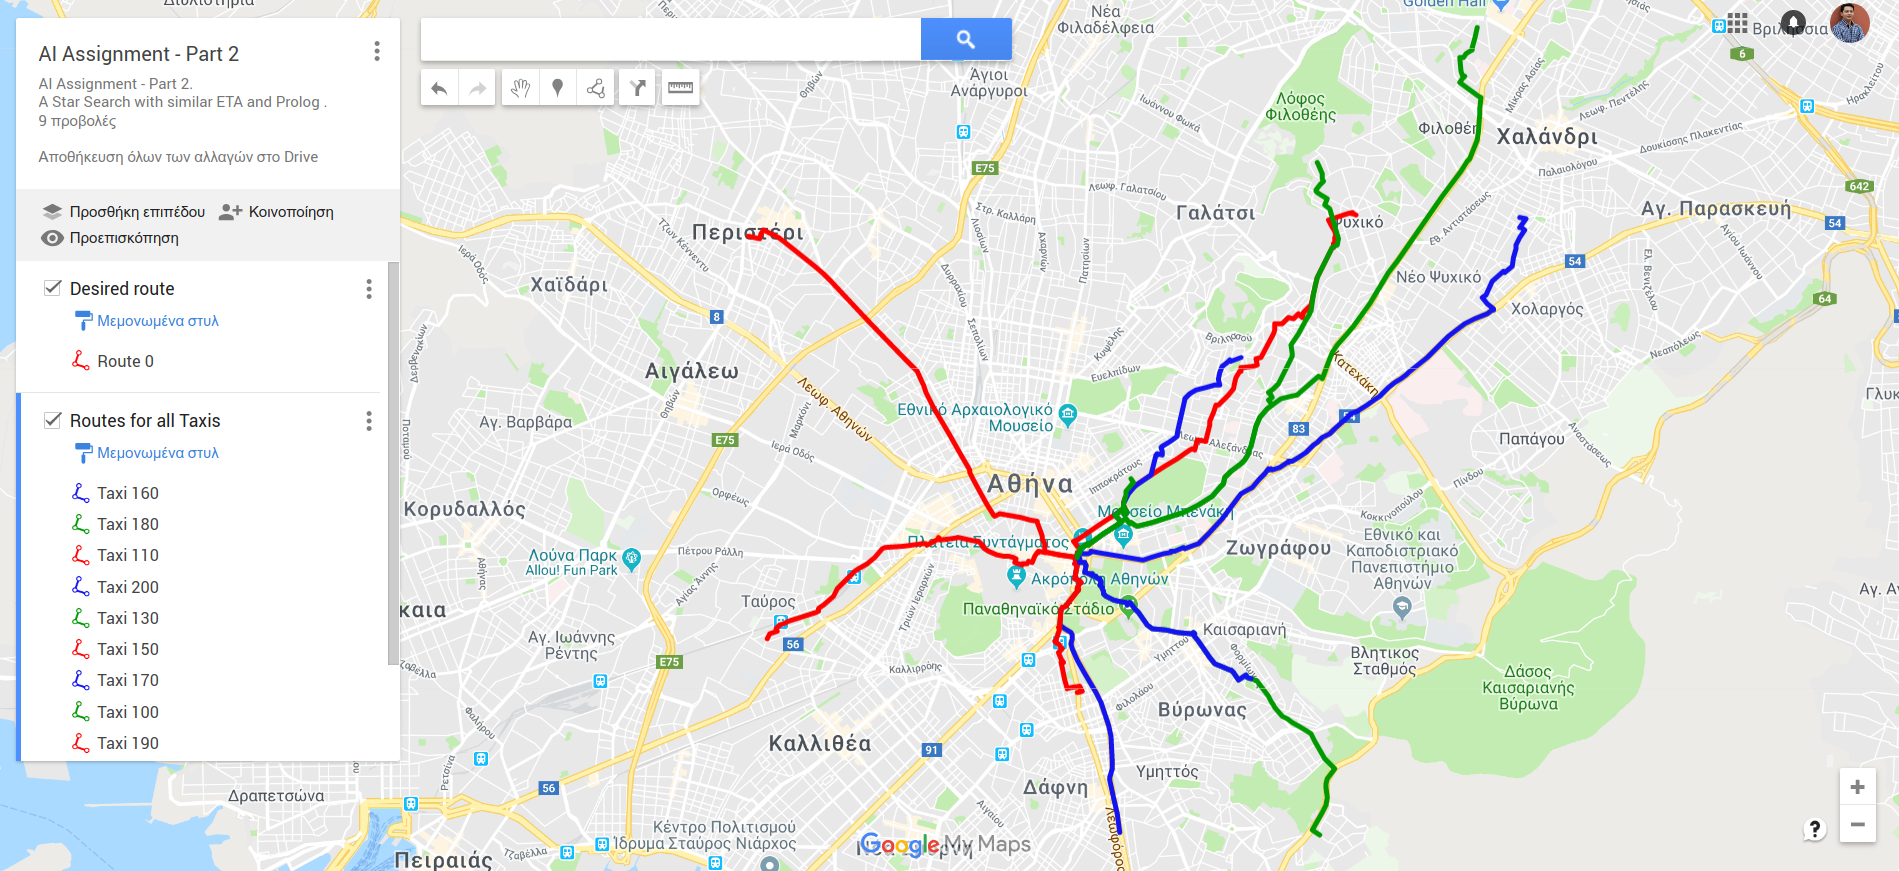
\includegraphics[scale=0.25]{example.png}
\caption{Αποτελέσματα διαδρομών για μηδενικό tolerance για όλα τα ταξί}
\label{}
\end{figure}

Οι δύο κατατάξεις βρίσκονται στην προηγούμενη ενότητα της αναφοράς.

Τα KML αρχεία βρίσκονται στη διαδρομή \texttt{lab2/results/\{route, taxis\}\{tol\}.kml}.




\begin{thebibliography}{9}

\bibitem{norvig} Russell, Stuart J., and Peter Norvig. Artificial intelligence: a modern approach. Malaysia; Pearson Education Limited,, 2016.

\bibitem{stamou} Στάμου Γ., Τεχνητή Νοημοσύνη, Διαφάνειες

\end{thebibliography}

\end{document}
